

\documentclass[5pt]{article}

\usepackage{sectsty}
\usepackage{graphicx}
\usepackage{lipsum} % for generating dummy text
\usepackage[margin=1in]{geometry}
\usepackage{setspace}
\usepackage{array}
\usepackage{cellspace}
\usepackage{tabularx}
\usepackage[table]{xcolor}
\usepackage{tabularray}
\usepackage{pgfplots}


\usepackage{hyperref}
\usepackage{scrextend}
\graphicspath{ {../assets} }

\usepackage[italian]{babel}


% package and setup for tables
\usepackage{float}
\usepackage[table]{xcolor}
\renewcommand{\arraystretch}{1.5}
\arrayrulecolor{black}


% Margins
\topmargin=-0.45in
\evensidemargin=0in
\oddsidemargin=0in
\textwidth=6.5in
\textheight=9.0in
\headsep=0.25in

\setlength{\parindent}{0pt}

\title{Specifica Tecnica}
\author{Jackpot Coding}
\renewcommand*\contentsname{Indice}
\date{\today}
%STARTOF THE DOCUMENT
\begin{document}
	
	%-------------------------
	
	% Reduce top margin only on the first page
	\newgeometry{top=0.5in}
	
	%UNIPD LOGO
	\vspace{8pt}
		
\includegraphics[scale=0.2]{UNIPDFull.png}
	%END UNIPD LOGO
	
	\vspace{30pt}
	
	%COURSE INFO
	\begin{minipage}[t]{0.48\textwidth}
		%COURSE TITLE
		\begin{flushleft}
			Informatica\\
			\vspace{5pt}
			\textbf{\LARGE Ingegneria del Software}\\
			Anno Accademico: 2023/2024
		\end{flushleft}
		%END COURSE TITLE
	\end{minipage}
	%END COURSE INFO
	
	
	\vspace{5px}
	
	
	%BLACK LINE
	\rule{\textwidth}{5pt}
	
	%JACKPOT CODING INFO
	\begin{minipage}[t]{0.50\textwidth}
		%LOGO JACKPOT CODING
		\begin{flushleft}
			\hspace{10pt}
				
\includegraphics[scale=0.65]{jackpot-logo.png} 
		\end{flushleft}
	\end{minipage}
	\hspace{-60pt} % This adds horizontal space between the minipages
	\begin{flushright}
		\begin{minipage}[t]{0.50\textwidth}
			%INFO JACKPOT CODING
			\begin{flushright}
				Gruppo: {\Large Jackpot Coding}\\
				Email: \href{mailto:jackpotcoding@gmail.com}{jackpotcoding@gmail.com}
			\end{flushright}
		\end{minipage}
	\end{flushright}
	%END JACKPOT CODING INFO
	
	\vspace{24pt}
	
	%TITLE
	\begin{center}
		\textbf{\LARGE SPECIFICA TECNICA}
	\end{center}
	%END TITLE
	
	\vspace{13pt}
	
	\begin{flushleft}
		\begin{spacing}{1.5}
			DESTINATARI: Prof. T. Vardanega, Prof. R. Cardin\\%INSERT HERE THE NAMES
		\end{spacing}
	\end{flushleft}
	
	\begin{flushright}
		\begin{spacing}{1}
			USO: ESTERNO\\
			VERSIONE: 1.0.0\\
		\end{spacing}
	\end{flushright}
	
	
	% Restore original margins from the second page onwards
	\restoregeometry
	
	\pagebreak
	
	\textbf{\Large Registro delle modifiche}
	\begin{table}[H]
		\centering
		\rowcolors{2}{black!15}{}
		\resizebox{\linewidth}{!}{
			\begin{tabular}{|c|c|c|c|c|}
				\rowcolor{teal!50}
				\hline
				\textbf{Versione} & \textbf{Data} & \textbf{Autore} & \textbf{Verificatore} & \textbf{Modifica} \\
				\hline
				1.0.0 & 08/05/2024 & - & E. Gallo & Verifica documento\\
				\hline
				0.1.3 & 08/05/2024 & G. Moretto & E. Gallo & Aggiunta indicazione termini presenti nel Glossario\\
				\hline
				0.1.2 & 06/05/2024 & G. Moretto & E. Gallo & Aggiunta CSVParser e miglioramento descrizioni delle classi \\
				\hline
				0.1.1 & 03/05/2024 & E. Gallo & G. Moretto & Sistemato \textit{Design pattern} utilizzati - \textit{Strategy} \\
				\hline
				0.1.0 & 03/05/2024 & - & E. Gallo & Verifica documento \\
				\hline
				0.0.15 & 28/04/2024 & G.Moretto & E. Gallo & Aggiunta di SonarQube come strumento di testing \\
				\hline
				0.0.14 & 25/04/2024 & R. Simionato & G.Moretto & Aggiunta dei riferimenti al Glossario \\
				\hline
				0.0.13 & 23/04/2024 & G. Moretto & R. Simionato & Aggiunta QueryForm, QueryGenerationView, QueryGenerator, sostituito Tensorflow con Torch \\
				\hline
				0.0.12 & 21/04/2024 & G. Moretto & R. Simionato & Aggiornamento diagramma Views con nuova operazione per PromptCreator\\
				\hline
				0.0.11 & 18/04/2024 & G. Moretto & R. Simionato & Aggiunta dei digrammi delle classi\\
				\hline
				0.0.10 & 10/04/2024 & G. Moretto & R. Simionato & Aggiunta dello strumento di testing coveralls.io\\
				\hline
				0.0.9 & 09/04/2024 & - & G. Moretto & Documento rinominato in "Specifica Tecnica"\\
				\hline
				0.0.8 & 09/04/2024 & E. Gallo & G. Moretto & Aggiunti riferimenti normativi ed informativi \\ 
				\hline
				0.0.7 & 06/04/2024 & M. Favaretto & G. Moretto & Aggiunta sezione \textit{Design pattern} utilizzati - \textit{M.V.T.} \\ 
    			\hline
    			0.0.6 & 05/04/2024 & E. Gallo & M. Favaretto & Aggiunta sezione Design pattern utilizzati - Strategy \\
    			\hline
				0.0.5 & 04/04/2024 & M. Camillo & E. Gallo & Introduzione Documento \\
                \hline
				0.0.4 & 04/04/2024 & M. Gobbo & E. Gallo & Introduzione all'architettura \\
				\hline
				0.0.3 & 03/04/2024 & G. Moretto & M. Gobbo & Aggiunto elenco delle tabelle \\
				\hline
				0.0.2 & 02/04/2024 & G. Moretto & M. Gobbo & Aggiunta tabelle tecnologie codifica e testing \\
				\hline
				0.0.1 & 27/03/2024 & G. Moretto & M. Gobbo & Aggiunta struttura documento \\
				\hline
			\end{tabular}
		}
		\label{tab:conference}
	\end{table}
	
	\pagebreak
	\tableofcontents
	\pagebreak
	\textbf{\Large Elenco delle immagini} \\
	\makeatletter
	\@starttoc{lof}% Print List of Figures
	\makeatother
	
	\pagebreak
	\textbf{\Large Elenco delle tabelle} \\
	\makeatletter
	\@starttoc{lot}% Print List of Tables
	\makeatother
	\pagebreak
	
	\section{Introduzione}
	
	\subsection{Scopo del Documento}

    Il documento ha lo scopo di presentare e motivare le scelte architetturali e di design applicate al prodotto, oltre che a fornire una lista completa delle tecnologie utilizzate. La struttura interna del prodotto è esposta all'interno del documento sotto forma di diagramma delle classi, in maniera da rendere più chiaro il \textit{software}\textsuperscript{G} sviluppato. Vengono inoltre approfonditi e motivati a loro volta i design pattern\textsuperscript{G} utilizzati. 
	
	\subsection{Scopo del Prodotto}
    Il capitolato\textsuperscript{G} proposto dall'azienda \textit{Zucchetti S.p.A.} ha come obiettivo la realizzazione di un applicativo web al fine di studiare la fattibilità di un prodotto che possa elaborare una frase in linguaggio naturale\textsuperscript{G}. Questa frase, anche se fornita da un utente\textsuperscript{G} inesperto, deve generare come output una \textit{query} SQL\textsuperscript{G} in grado di interrogare un database\textsuperscript{G} (di cui è conosciuta la struttura) in modo efficiente e affidabile.
	
	\subsection{Glossario}
    Al fine di evitare ambiguità o incomprensioni relative alla terminologia usata all'interno del documento, è fornito un \textit{Glossario} in cui vengono riportate definizioni precise per ogni termine potenzialmente ambiguo. La presenza di tali termini all'interno del documento è indicata con la presenza, vicino alla voce, di una \textit{G} in apice ($^G$). 
	\subsection{Riferimenti}
	\subsubsection{Riferimenti normativi}
	\begin{itemize}
		\item Capitolato\textsuperscript{G} C9 - \textit{ChatSQL} \\ \url{https://www.math.unipd.it/~tullio/IS-1/2023/Progetto/C9.pdf}
		\item Norme di progetto\textsuperscript{G} V1.0.2
		\item Glossario V1.0.0 \\
		\url{https://jackpot-coding.github.io/chatSQL/docs/esterni/glossario_v1.0.0.pdf}
	\end{itemize}
	\subsubsection{Riferimenti informativi}
	Slide del corso Ingegneria del Software:
	\begin{itemize}
		\item Progettazione software \\
		\url{https://www.math.unipd.it/~tullio/IS-1/2023/Dispense/T6.pdf}
		\item Diagramma delle classi \\
		\url{https://www.math.unipd.it/~rcardin/swea/2023/Diagrammi%20delle%20Classi.pdf}
		\item Pattern MVC e derivati \\
		\url{https://www.math.unipd.it/~rcardin/sweb/2022/L02.pdf}
		\item SOLID programming \\
		\url{https://www.math.unipd.it/~rcardin/swea/2021/SOLID%20Principles%20of%20Object-Oriented%20Design_4x4.pdf}
		\item Pattern comportamentali \\
		\url{https://www.math.unipd.it/~rcardin/swea/2021/Design%20Pattern%20Comportamentali_4x4.pdf}
	\end{itemize}
	
	\section{Tecnologie}
	
	\subsection{Codifica}

	\begin{longtblr}[
			caption = {Tecnologie di codifica.},
		]
		{
			colspec={|Q[0.15\linewidth]|Q[0.15\linewidth]|Q[0.70\linewidth]|},
			rows={halign=l},
			column{1}={halign=c},
			column{2}={halign=c},
			column{3}={halign=l},
			row{1}={halign=c},
			row{odd} = {gray!20},
			row{1}={teal!50},
			row{2}={teal!50},
			row{6}={teal!50},
			row{10}={teal!50}
		}
	
		\hline
		\textbf{Tecnologia} & \textbf{Versione} & \textbf{Descrizione} \\
		\hline
		\SetCell[c=3]{c} \textbf{Linguaggi} \\
		\hline
		HTML\textsuperscript{G} & 5 & Linguaggio di \textit{markup} utilizzato per la definizione della struttura di pagine \textit{web} \\
		\hline
		CSS\textsuperscript{G} & 3 & Linguaggio utilizzato per applicare stile a elementi presenti in una pagina HTML \\
		\hline
		Python & 3.11.8 & Linguaggio di programmazione ad alto livello, orientato agli oggetti. Viene utilizzato per la creazione del \textit{server}. \\
		\hline
		\SetCell[c=3]{c} \textbf{Framework\textsuperscript{G} e Librerie\textsuperscript{G}} \\
		\hline
		Django & 5.0.3 & \textit{Framework} per la creazione di applicazioni \textit{web}, scritto in linguaggio \textit{Python}. \\
		\hline
		Torch & 2.2.2 & Libreria \textit{Python}\textsuperscript{G} per l'apprendimento automatico. \\
		\hline
		Transformers & 4.29.3 & Libreria \textit{Python}\textsuperscript{G} per l'utilizzo di modelli del portale \textit{Hugging Face} utilizzando \textit{Torch}\\
		\hline
		\SetCell[c=3]{c} \textbf{Strumenti} \\
		\hline
		Pip & 24.0 & Strumento per la gestione dei pacchetti utilizzati da applicazioni \textit{Python}\textsuperscript{G}.\\
		\hline
		Git & 2.44.0 & Strumento per il controllo di versione utilizzato per la gestione della \textit{repository}\textsuperscript{G} remota presente su \textit{GitHub}\textsuperscript{G}. \\
		\hline
	\end{longtblr}
	
	\subsection{Testing}
	\begin{longtblr}[
		caption = {Tecnologie di testing.},
		]
		{
			colspec={|Q[0.15\linewidth]|Q[0.15\linewidth]|Q[0.70\linewidth]|},
			rows={halign=l},
			column{1}={halign=c},
			column{2}={halign=c},
			column{3}={halign=l},
			row{1}={halign=c},
			row{odd} = {gray!20},
			row{1}={teal!50},
			row{2}={teal!50},
			row{8}={teal!50}
		}
		\hline
		\textbf{Tecnologia} & \textbf{Versione} & \textbf{Descrizione} \\
		\hline
		\SetCell[c=3]{c} \textbf{\textit{Framework}\textsuperscript{G} e Librerie\textsuperscript{G}} \\
		\hline
		\textit{Unittest} & 3.11.8 & \textit{Framework} incluso nel linguaggio \textit{Python}\textsuperscript{G} utilizzato per il \textit{testing} di unità, utilizzato dal \textit{framework Django}.\\
		\hline
		\textit{Django Test Client} & 5.0.3 & \textit{Client} per il \textit{testing} di un applicazione \textit{web} simulando un \textit{browser}\textsuperscript{G}, integrato nel \textit{framework}\textsuperscript{G} Django.\\
		\hline
		\textit{coverage.py} & 7.4.4 & \textit{Tool} per misurare il \textit{code coverage}\textsuperscript{G} in applicazioni \textit{Python}\textsuperscript{G} integrabile nel \textit{framework Django}. \\
		\hline
		\textit{Prospector} & 1.10.3 & \textit{Tool} per l'analisi statica di codice scritto nel linguaggio \textit{Python}\textsuperscript{G}. \\
		\hline
		\textit{SonarQube} & 10.5 & \textit{Tool} per l'analisi automatica della qualità del codice in vari linguaggi e \textit{framework}\textsuperscript{G}.\\
		\hline
		\SetCell[c=3]{c} \textbf{Strumenti} \\
		\hline
		\textit{GitHub Actions} & - & Servizio di \textit{Github}\textsuperscript{G} per la \textit{Continuous Integration}, automatizza i processi di \textit{build, test e deploy} del prodotto \textit{software}\textsuperscript{G}.\\
		\hline
		\textit{Coveralls.io} & - & Servizio per la visualizzazione dei rapporti di \textit{code coverage}\textsuperscript{G} e applicazione di un \textit{badge} alla \textit{repository}\textsuperscript{G}.\\
		\hline
	\end{longtblr}
	
	\section{Architettura}
	
	\subsection{Introduzione}
L'architettura di \textit{"Chat SQL"} si basa sul \textit{design pattern}\textsuperscript{G} architetturale \textit{MVT(Model View Template)}.\\

In questo \textit{pattern}, il \textit{"Model"} rappresenta i dati e la logica di \textit{business} dell'applicazione, la \textit{"View"} esegue la \textit{business logic}, interagisce con il \textit{Model} e ritorna risposte Http, infine  il \textit{"Template"} definisce la struttura dell'interfaccia utente e come i dati vengono visualizzati al suo interno. Più nello specifico il \textit{"Template"}, nel caso della nostra applicazione, definisce la struttura di documenti HTML\textsuperscript{G}.\\

Questo \textit{design pattern}\textsuperscript{G} è simile a \textit{MVC(Model View Controller)} \\\\
E' stata scelta questa architettura sia perché dettata dal \textit{framework} sia in quanto offre i seguenti vantaggi:
\begin{itemize}
    \item \textbf{Separazione delle responsabilità}: \textit{MVT} separa chiaramente le responsabilità tra \textit{Model}, \textit{View} e \textit{Template}. Questo permette una migliore organizzazione del codice, facilitando la manutenzione e la scalabilità dell'applicazione.

    \item \textbf{Riutilizzo dei template}: I \textit{template} in \textit{MVT} consentono di separare la presentazione dalla logica di \textit{business}. Ciò facilita il riutilizzo dei componenti di interfaccia utente in diverse parti dell'applicazione, riducendo la duplicazione del codice e migliorando l'efficienza dello sviluppo.

    \item \textbf{Aumento delle Performance}: Utilizzare i \textit{template} pre-renderizzati può migliorare le prestazioni dell'applicazione rispetto a un'architettura \textit{MVC} tradizionale, poiché il \textit{rendering} dei \textit{template} può essere più efficiente rispetto ad esempio alla generazione dinamica di HTML\textsuperscript{G} lato \textit{server}.

\end{itemize}
	
	\subsection{Diagrammi delle classi}
	
	\subsubsection{Modelli}
	
	\begin{figure}[H]
		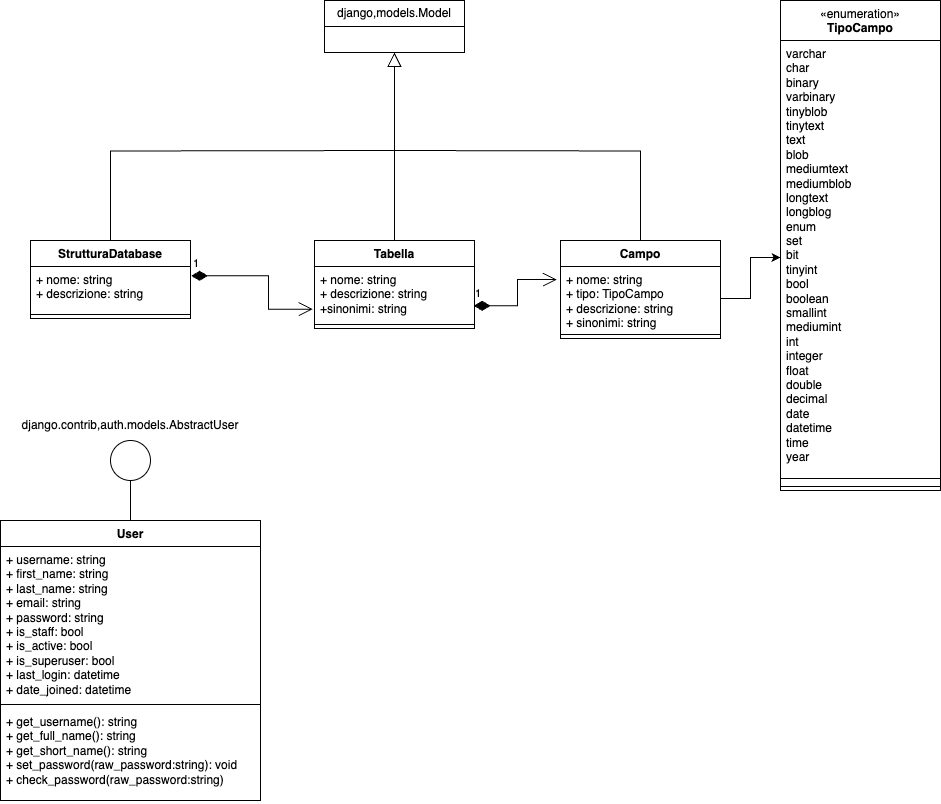
\includegraphics[scale=0.55]{UML_classes/models.png}
		\caption{Diagramma UML delle classi Model}
		\centering
	\end{figure}	
	
	Il compito del modello è quello di gestire i dati che vengono utilizzati dall'applicazione. Formano la struttura dei dati dell'intera applicazione e sono rappresentati in un \textit{database}\textsuperscript{G}.\\
	
	I modelli definiti derivano dalla classe Model fornita dal \textit{framework}\textsuperscript{G} Django e sono:
	\begin{itemize}
		\item \textbf{StrutturaDatabase}: rappresenta le varie strutture \textit{database}\textsuperscript{G} definite dall'amministratore\textsuperscript{G};
		\item \textbf{Tabella}: rappresenta le tabelle che compongono una Struttura \textit{Database}\textsuperscript{G};
		\item \textbf{Campo}: rappresenta i campi che compongono una Tabella\textsuperscript{G}. Questo utilizza un enumerazione chiamata TipoCampo che indica le tipologie di campo selezionabili;
	\end{itemize}
	
	Viene inoltre utilizzato il modello User fornito dal \textit{framework}\textsuperscript{G} Django del quale si elencano gli attributi e operazioni più rilevanti.\\
	
	
	\subsubsection{View}
	
	\begin{figure}[H]
		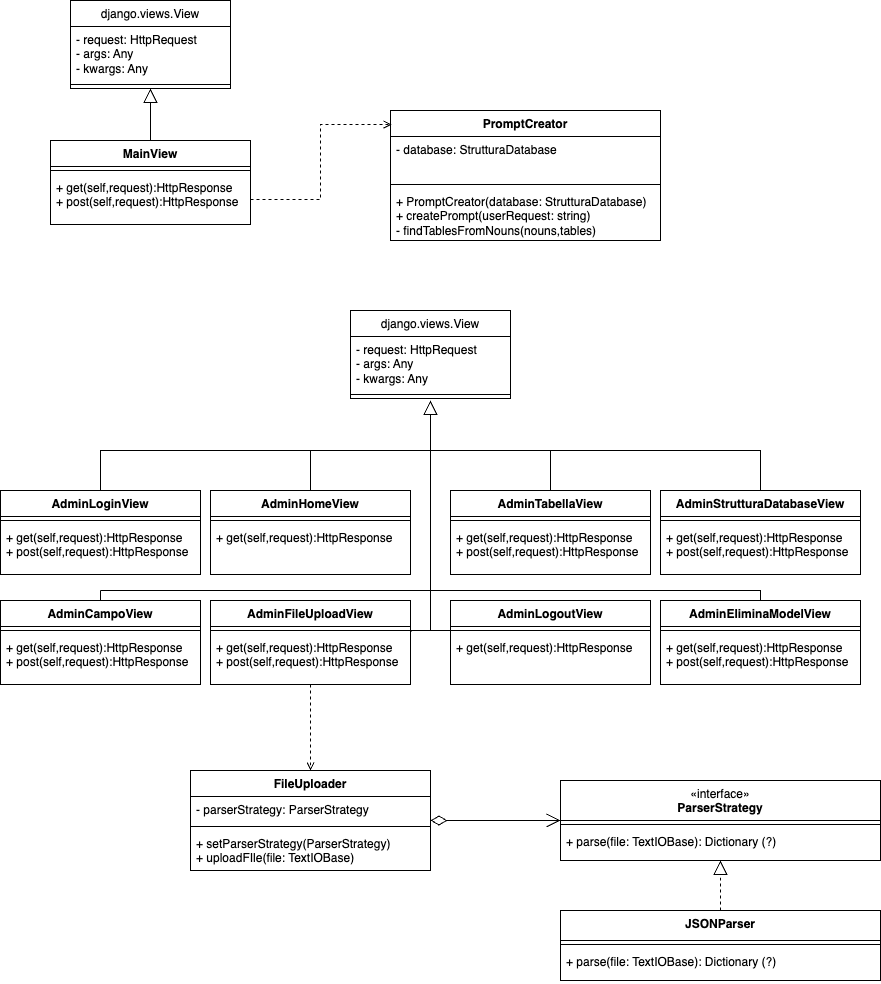
\includegraphics[scale=0.50]{UML_classes/views.png}
		\caption{Diagramma UML delle classi View}
		\centering
	\end{figure}

	
	Il compito delle \textit{view} è quella di ricevere richieste dal \textit{browser}\textsuperscript{G} e di restituire risposte sottoforma di pagine HTML\textsuperscript{G} o altri elementi che possono essere visualizzati da un \textit{browser}.\\
	
	Le \textit{view} definite derivano dalla classe \textit{View} fornita dal \textit{framework}\textsuperscript{G} Django e sono divise per area principale e area amministrativa.\\
	
	Le \textit{view} dell'area principale sono:
	\begin{itemize}
		\item  \textbf{MainView}: si occupa di ricevere la richiesta di generazione del \textit{prompt}\textsuperscript{G} dall'utente\textsuperscript{G} e di restituirlo. Per fare questo utilizza una classe chiamata PromptCreator che si occupa di generare il prompt per la richiesta ricevuta dalla view;
		\item \textbf{PromptCreator}: si occupa di creare il \textit{prompt}\textsuperscript{G} a partire dalla struttura \textit{database}\textsuperscript{G} e dalla frase in linguaggio naturale\textsuperscript{G} fornita;
		\item \textbf{QueryGenerationView}: si occupa di ricevere il \textit{prompt}\textsuperscript{G} generato, inviarlo al modello \textit{LLM}\textsuperscript{G} esterno tramite la classe Querygenerator e ritornare la risposta;
		\item \textbf{QueryGenerator}: si occupa di generare la \textit{query} SQL\textsuperscript{G} richiesta inviando il \textit{prompt}\textsuperscript{G} generato ad un servizio \textit{LLM}\textsuperscript{G} esterno.
	\end{itemize}

	
	Le view dell'area amministrativa sono:
	\begin{itemize}
		\item \textbf{AdminLoginView}: responsabile per l'autenticazione dell'amministratore\textsuperscript{G};
		\item \textbf{AdminLogoutView}: responsabile per il \textit{logout} dell'amministratore\textsuperscript{G};
		\item \textbf{AdminHomeView}: resituisce la pagina home dell'area amministrativa dove è presente la lista delle Strutture Database e il link per la creazione delle stesse;
		\item \textbf{AdminStrutturaDatabaseView}: restituisce la pagina di creazione e modifica della StrutturaDatabase e la lista delle tabelle che la compongono;
		\item \textbf{AdminTabellaView}: restituisce la pagina di creazione e modifica delle Tabelle e la lista dei campi che la compongono;
		\item \textbf{AdminCampoView}: restituisce la pagina di creazione e modifica dei Campi di una Tabella\textsuperscript{G};
		\item \textbf{AdminFileUploadView}: restituisce la pagina per il caricamento di un \textit{file}\textsuperscript{G} di struttura \textit{database}\textsuperscript{G} (con eventuale messaggio di errore o successo a seconda dell'esito del caricamento) e utilizza la classe FileUploader per la conversione ed il salvataggio come StrutturaDatabase;
		\item \textbf{FileUploader}: responsabile per il caricamento di file che rappresentano una struttura \textit{database}\textsuperscript{G}, utilizza l'interfaccia \textbf{ParserStrategy}  che viene implementata con le classi:
		\begin{itemize}
			\item \textbf{JSONParser}: per importare \textit{file}\textsuperscript{G} JSON con struttura nota;
			\item \textbf{CSVParser}: per importare \textit{file} CSV con struttura nota;
		\end{itemize}
		Ognuno di questi \textit{parser} restituisce, a seconda dell'esito, un messaggio di errore o successo contenuto nell'enumerazione \textbf{ParserStatus};
		\item \textbf{AdminEliminaModelView}: responsabile per l'eliminazione di un oggetto dal \textit{database}\textsuperscript{G} dato il suo id ed il suo modello. Restituisce una pagina per la conferma dell'eliminazione e l'eliminazione stessa.
	\end{itemize}
	
	\subsubsection{Form}
	\begin{figure}[H]
			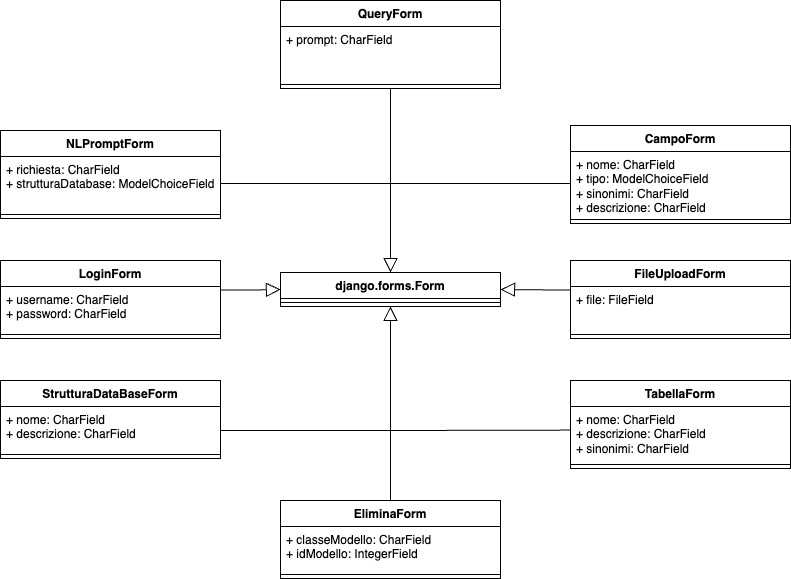
\includegraphics[scale=0.65]{UML_classes/forms.png}
			\caption{Diagramma UML delle classi Form}
			\centering
	\end{figure}

	Il compito delle classi \textit{form}\textsuperscript{G} e quella di definire \textit{form} HTML\textsuperscript{G} sottoforma di classe. Questo per utilizzare le funzioni di validazione e gestione fornite dal \textit{framework}\textsuperscript{G} Django tramite la classe Form dalla quale derivano i \textit{form} da noi definiti:
	\begin{itemize}
		\item \textbf{NLPromptForm}: raccoglie i dati per la generazione del \textit{prompt}\textsuperscript{G}, da sottoporre poi ad un \textit{LLM}\textsuperscript{G};
		\item \textbf{QueryForm}: raccoglie i dati per la generazione della \textit{query} SQL\textsuperscript{G};
		\item \textbf{LoginForm}: raccoglie i dati per il \textit{login}\textsuperscript{G} dell'amministratore\textsuperscript{G};
		\item \textbf{StrutturaDatabaseForm}: raccoglie i dati per la creazione e modifica di una Struttura Database;
		\item \textbf{TabellaForm}: raccoglie i dati per la creazione e modifica di una Tabella\textsuperscript{G};
		\item \textbf{CampoForm}: raccoglie i dati per la creazione e modifica di un Campo;
		\item \textbf{UploadFileForm}: raccoglie i dati per il caricamento del \textit{file}\textsuperscript{G} di struttura \textit{database}\textsuperscript{G};
		\item \textbf{EliminaForm}: raccoglie i dati per l'eliminazione di un oggetto dal \textit{database}\textsuperscript{G};
	\end{itemize}
	
	\subsection{Design pattern utilizzati}
			\subsubsection{Model-View-Template}
			% eventuale immagine mvt
			Per lo sviluppo del prodotto, il gruppo ha scelto l'utilizzo del \textit{framework}\textsuperscript{G} Django. Il \textit{framework} propone un'architettura integrata,
			basata su una generalizzazione della \textit{view}, attraverso il \textit{design pattern}\textsuperscript{G} MVT. \\
			L'architettura proposta da \textit{Django} si compone di:
			\begin{itemize}
			\item \textit{File}\textsuperscript{G} per la gestione dei Modelli ;
			\item \textit{File} per la gestione delle \textit{View};
			\item \textit{File} per le impostazioni del progetto;
			\item \textit{File} per la configurazione degli URL;
			\item \textit{File} di \textit{template} per la definizione dell'interfaccia utente;
			\item \textit{File} per la gestione dei \textit{form}; 
			\item \textit{File} per la gestione dei test;
			\item Cartella contenente le migrazioni verso il sistema di \textit{database}\textsuperscript{G} scelto;
			\item Cartella contenente \textit{file} statici come fogli di stile e immagini;
			\item Cartella per ogni applicazione che compone il prodotto;
			\end{itemize}

		\subsubsection{Strategy}
			% Immagine Design Pattern Strategy%
			Uno dei \textit{design pattern}\textsuperscript{G} comportamentali scelto dal gruppo è lo \textit{Strategy}\textsuperscript{G}. 
			In particolare, viene integrato per permettere al programma di riconoscere diversi tipi di \textit{file}\textsuperscript{G} quando viene eseguito \textit{l'upload}. In base all'estensione del \textit{file}, il programma sceglie quale strategia utilizzare per raccogliere ed immagazzinare nel migliore dei modi le informazioni caricate.
			Al lato pratico, una volta caricato un \textit{file} tramite la classe \textit{FileUploader}, questo viene passato ad un'interfaccia che verrà successivamente implementata dalle classi:
			\begin{itemize}
				\item \textit{JSONParser}: per i \textit{file} di tipo JSON
				\item \textit{CSVParser}: per i \textit{file} CSV
			\end{itemize} 
			Il gruppo ha poi individuato altri ambiti in cui un \textit{Design Pattern}\textsuperscript{G} \textit{Strategy} sarebbe ottimale. Per una questione di tempo principalmente, non sono stati implementati. Siccome il prodotto deve lavorare a stretto contatto con gli \textit{LLM}\textsuperscript{G}, sarebbe utile che la loro chiamata venga effettuata solo quando necessario, senza usare i modelli più grandi per richieste piccole.  \\
	
\end{document}
